% \lipsum[4] Citing \cite{InfH} properly.
% Was ist eine \gls{guid}?
% Eine \gls{guid} kollidiert nicht gerne.

% Kabellose Technologien sind in abgelegenen Gebieten wichtig \cite{APCW2006}.

sys diagram
% todo: add systemarchitektur_diagram
% 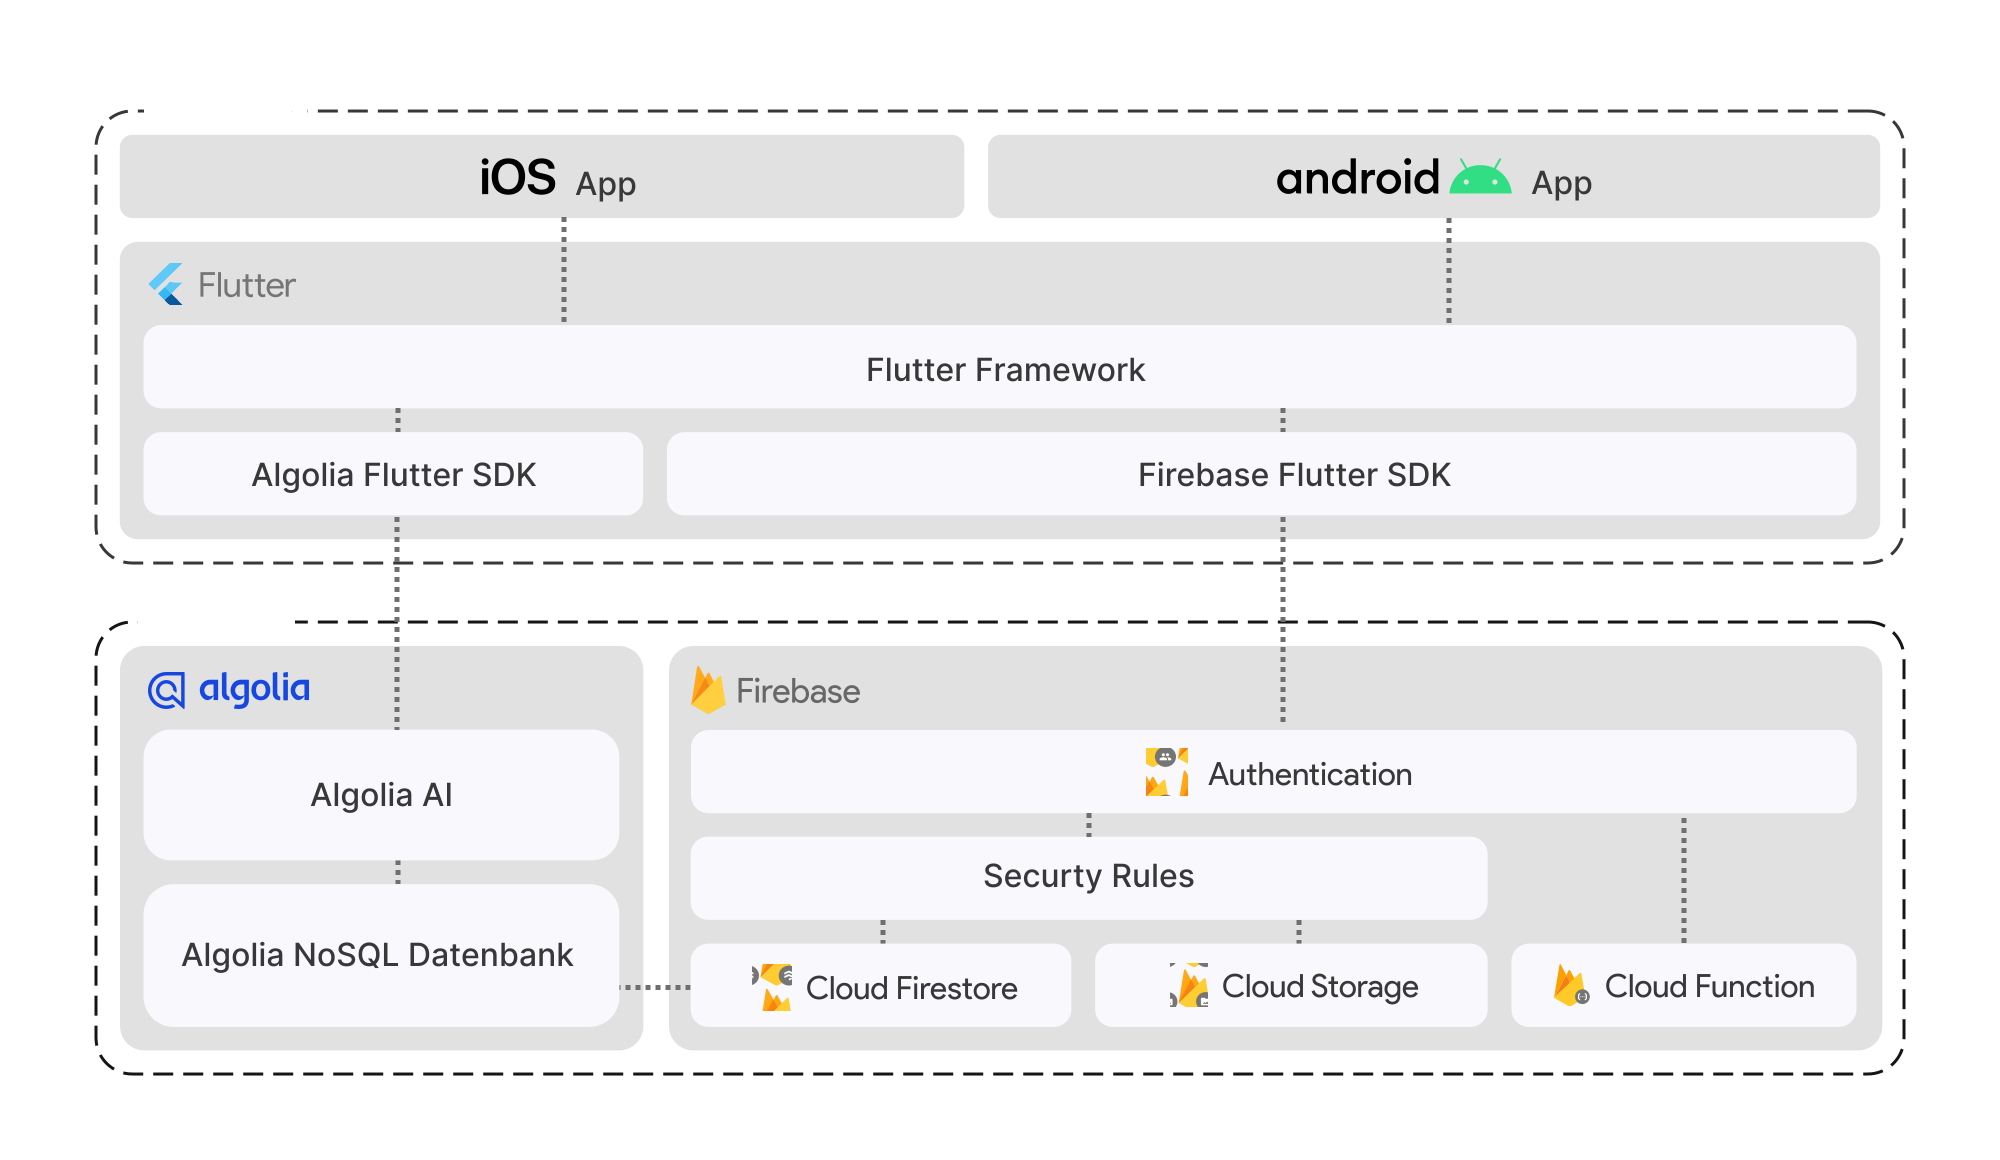
\includegraphics[width=0.2\textwidth]{pics/systemarchitektur_diagram.svg}

% \includesvg{pics/systemarchitektur_diagram.svg}


\section{Flutter}

Hier kommt die Beschreibung der Technologie und deren Vorteile/Nachteile, auf Basis von wissenschaftlichen Studien und Erfahrungen aus der Praxis.

Quellen:

https://docs.flutter.dev/resources/architectural-overview

https://flutter.dev/docs/resources/technical-overview,
https://pub.dev/packages/flutter


% \subsection{iOS}
% \subsubsection{CI/CD}

% \subsection{Android}
% \subsubsection{CI/CD}
% \subsubsection{Firebase App Distribution}




\section{Firebase}
\author{Martin Hausleitner}


Hier wird die Vorstellung der Firebase Technologie inklusive deren Funktionen und Vorteile erklärt.

Quellen:

https://firebase.google.com/docs/guides

https://medium.com/flutter-community/flutter-firebase-from-scratch-28c8ba7d98b5

\subsection{Firebase Authentication}

Beschreibung der Firebase Authentication Technologie, inklusive Sicherheitsregeln und Best Practices.

Quellen:

https://firebase.google.com/docs/auth

https://medium.com/flutter-community/firebase-authentication-in-flutter-752d14209a8a

\subsubsection{Security Rules}
\author{Martin Hausleitner}
In unserer App ist die Sicherheit ein sehr wichtiger Faktor,
um die Vertraulichkeit und Integrität der Daten und der
Nutzer zu gewährleisten. Firebase bietet für seine
Cloud-basierten Datenbank- und Speicherlösungen - Cloud
Firestore und Cloud Storage - die sogenannten Security
Rules\cite{firebase-rules-docs}\cite{firestore-rules-firestore-nochba}\cite{storage-rules-storage-nochba}, um den Zugriff auf
die Daten und Ressourcen zu kontrollieren. Diese Regeln
definieren, wer auf welche Art und Weise auf welche Daten
zugreifen darf.

Die Security Rules für Cloud Firestore und Cloud Storage sind in einer eigenen Sprache geschrieben und werden serverseitig auf Firebase-Servern ausgeführt. Die Syntax basiert auf einer ähnlichen Struktur wie JSON und erlaubt komplexe Abfragen. Die Regeln können für eine bestimmte Sammlung oder einen bestimmten Pfad definiert werden und erlauben es, bestimmte Bedingungen für Lese- oder Schreibzugriffe zu definieren.


\begin{lstlisting}[language=Python,caption=Security Rules Beispiel]
    match /posts/{postId} {
        allow read: if request.auth.uid != null;
        allow write: if request.auth.uid == resource.data.author;
      }
\end{lstlisting}

Diese Regel definiert, dass jeder Nutzer Lesezugriff auf
alle Posts hat, aber nur der Autor des Posts ihn auch ändern
darf.

Insgesamt bieten die Security Rules für Cloud Firestore und Cloud Storage eine leistungsstarke und flexible Möglichkeit, die Zugriffsrechte auf die Daten und Ressourcen in einer Firebase-App zu steuern. Mit Hilfe der Security Rules können wir sicherstellen, dass die Daten ihrer Nutzer geschützt und nur von berechtigten Personen abgerufen oder geändert werden können.



\subsection{Cloud Firestore}

Vorstellung der Datenbanktechnologie Firestore

Quellen:

https://firebase.google.com/docs/firestore

https://medium.com/flutter-community/firebase-cloud-firestore-in-flutter-26c6e8c6f90c

\subsubsection{Datenmodel}

Hier kommt die Erklärung des Datenmodells in Firebase Firestore und dessen Auswirkungen auf die App-Architektur.

Quellen:

https://firebase.google.com/docs/firestore/data-model

https://www.raywenderlich.com/6628345-cloud-firestore-for-flutter-getting-started

Weitere wichtige punkte:

\begin{compactitem}
    \item Präsentation des eigenen Datenmodells in der Arbeit.
    \item Diagramme werden verwendet, um das Modell zu präsentieren und Entscheidungen zu erläutern und zu begründen.
    \item Anforderungen der App-Architektur werden dabei berücksichtigt werden.
    \item Performance, Skalierbarkeit und Strukturierung können thematisiert werden.
    \item Zur Veranschaulichung unserer eigenen Datenmodell-Entwicklung kann auf ein Beispiel-Datenmodell-Diagramm auf der offiziellen Firebase-Website verwiesen werden, welches uns als Orientierungshilfe diente.
\end{compactitem}

Beispiel-Datenmodell-Diagramm Quelle:

https://firebase.google.com/docs/firestore/data-model\#structure\_your\_data

\subsection{Cloud Storage}

Beschreibung der Cloud Storage Technologie in Firebase und deren Einsatz in der App.

Quellen:

https://firebase.google.com/docs/storage

https://medium.com/flutter-community/firebase-cloud-storage-in-flutter-flutter-an-firebase-tutorial-c5de7835c6cd

\subsection{Firebase Cloud Functions}
\author{Martin Hausleitner}


Erklärung der Cloud Functions Technologie in Firebase, inklusive Beispiele für deren Einsatz in der App.

Quellen:

https://firebase.google.com/docs/functions

https://medium.com/codeburst/organizing-your-firebase-cloud-functions-67dc17b3b0da

\section{Algolia Search}

Vorstellung der Algolia Search Technologie und deren
Integration in die App-Architektur.

Algolia AI

Quellen:

https://www.algolia.com/doc/

https://www.algolia.com/doc/guides/sending-and-managing-data/send-and-update-your-data/tutorials/firebase-algolia/

\subsubsection{Firebase Cloud Function}

Beschreibung der Firebase Cloud Functions und deren Rolle in der Algolia Integration.

Quellen:

https://firebase.google.com/docs/functions

https://www.algolia.com/doc/guides/sending-and-managing-data/send-and-update-your-data/tutorials/firebase-algolia/
